\documentclass[12pt,oneside]{scrartcl}

\usepackage{lmodern}

\usepackage[utf8]{inputenc}
\usepackage[english]{babel} %ngerman produces "Inhaltsverzeichnis"
\usepackage{graphicx}
\usepackage{wrapfig}
\usepackage{units}
\usepackage{todonotes}
\usepackage{hyperref}
\usepackage{natbib}
\usepackage{textcomp}

\renewcommand{\topfraction}         {0.70} % max fraction of page for floats at top
\renewcommand{\dbltopfraction}      {0.70} % for twocolumn layout, see topfraction above
\renewcommand{\bottomfraction}      {0.70} % max fraction of page for floats at bottom
\renewcommand{\textfraction}        {0.20} % min fraction of page for text
\renewcommand{\floatpagefraction}   {0.60} % min fraction of floatpage that should have floats
\renewcommand{\dblfloatpagefraction}{0.60} % for twocolumn layout, see floatpagefraction above
\setcounter{totalnumber} {6}               % max number of floats on a single page
\setcounter{topnumber}   {6}               % max number of top floats on a single page
\setcounter{dbltopnumber}{6}               % for twocolumn layout, see topnumber above
\setcounter{bottomnumber}{6}               % max number of bottom floats on a single page


\title{Progress report (TODO)}

\date{\today}

\author{
Matthias Ehrlich \and
Sebastian Jeltsch \and
Eric M\"uller \and
Sven Schrader \and
Bernhard Vogginger
}

\begin{document}
\maketitle

% ESTER could be
% Experimental Server             for Transaction-based Experiment Runs
% EUTER could be
% Experimental Userside interface for Transaction-based Experiment Runs

\section*{WP 3 Task 2: Software development for the HMF}

% TODO: Intro?

%\begin{wrapfigure}{r}{.5\textwidth} % force here (lower-case r)
\begin{figure}[ht!]
	\begin{center}
	%\fbox{
	%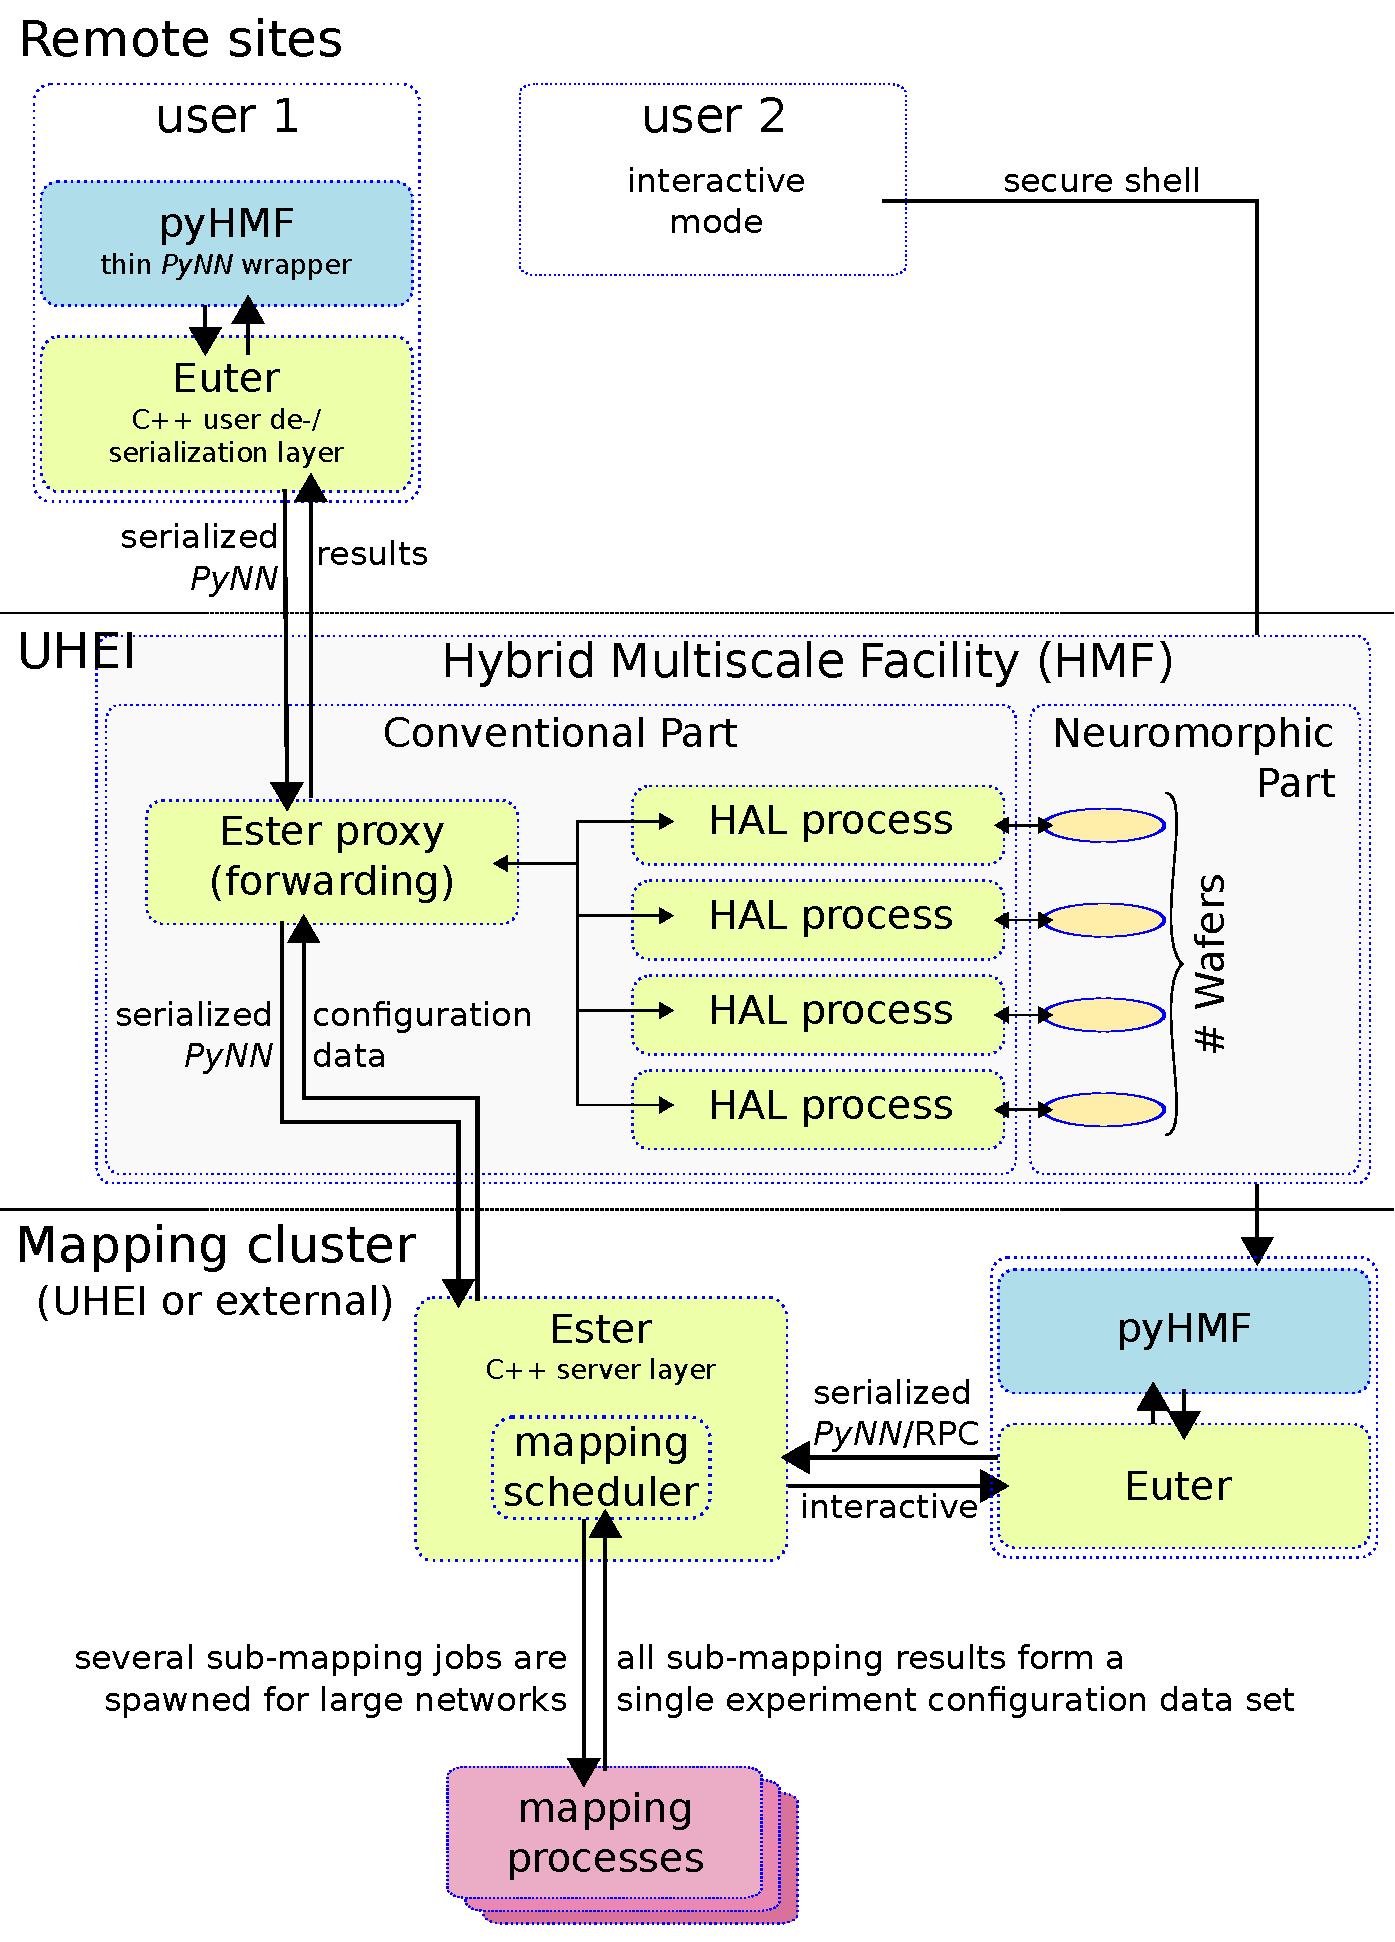
\includegraphics[width=.48\textwidth,clip]{arch_brainscales_progress.pdf}
	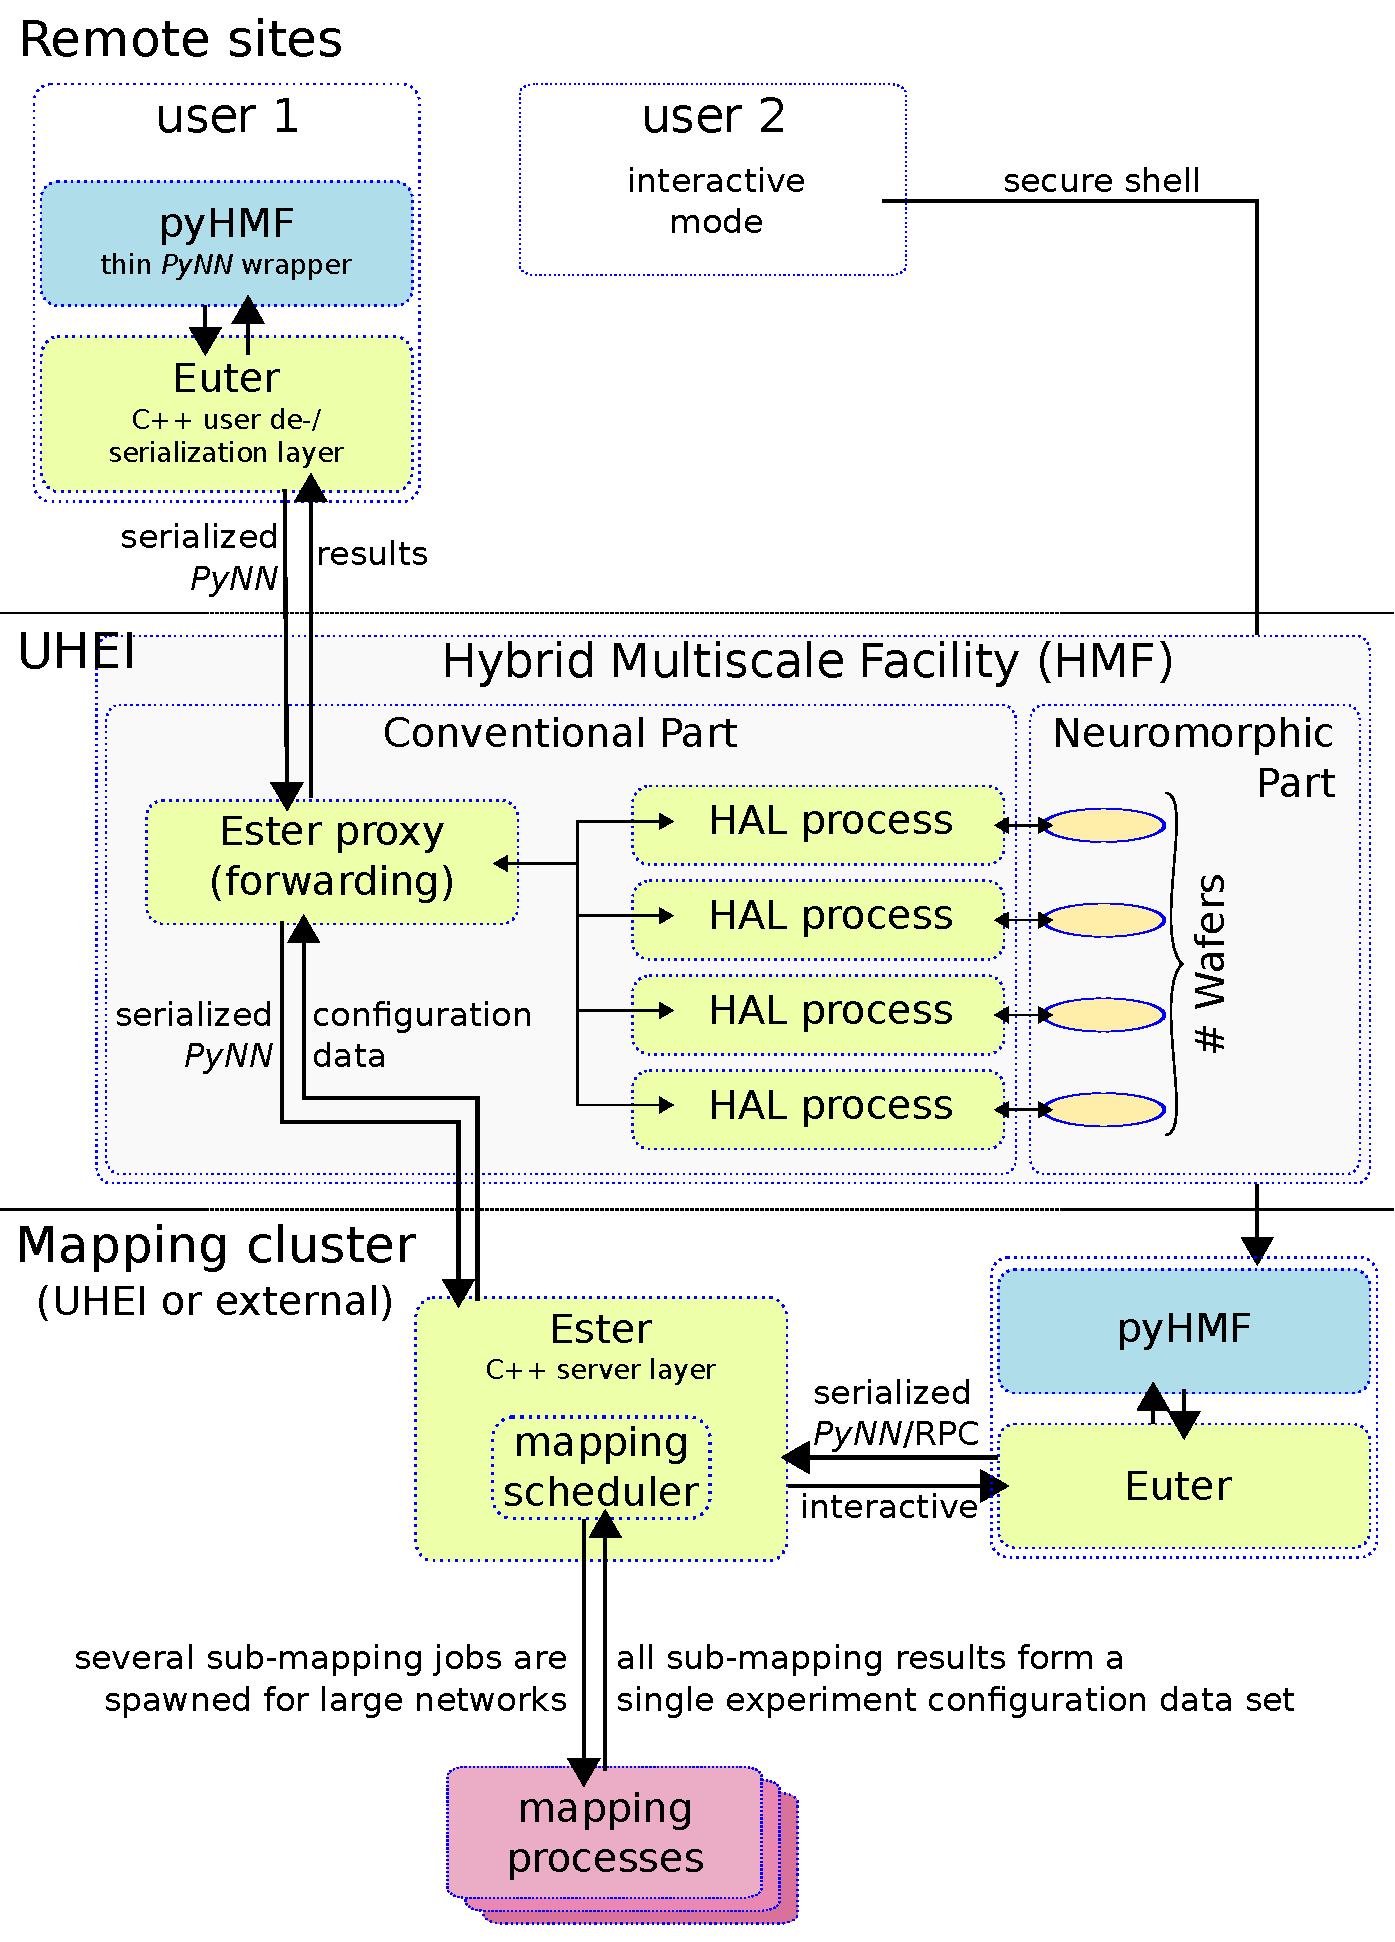
\includegraphics[height=.9\textheight,clip]{arch_brainscales_progress.pdf}
	%}
	\end{center}
	\caption{\label{fig:overview-ester}
	Overview of the new testbed for a scalable software framework.
	}
%\end{wrapfigure}
\end{figure}

Enabling users to efficiently emulate large neuronal network models spanning over multiple wafers on the HMF poses several new software challenges.
%
The full set of processes that will control the neuromorphic part of the HMF resembles the task of an operating system (OS) that controls the hardware of a common PC.
%
Its workflow is depicted in (Figure \ref{fig:overview-ester}) and has been developed in close collaboration with BrainScaleS' hardware-, software-, and modeling groups.


\subsection*{An OS for the HMF}

The major requirements for the new software framework are: (1) computing valid hardware configurations that represent the user's model.
(2) handling runtime data (mostly spikes) at high bandwidth and (3) providing many users in parallel an interface that fits their workflows.
%
In addition, users should be able to use a common neuronal network description language like \emph{PyNN} without the need to be concerned about hardware specifics.
%
In the following, a software framework is presented that tackles these challenges.

At the highest level, the user interacts with the \emph{PyNN} interface.
%
Below \emph{PyNN}, a thin adapter layer called \emph{pyHMF} translates between Python and the next (\texttt{C++}-based) layer.
%
This (cf.\ Figure \ref{fig:overview-ester}) so-called \emph{Euter} layer serializes the \emph{PyNN}-based network description into a binary format.
\emph{PyNN}'s \texttt{end()} function initiates the transfer to the \emph{Ester proxy} (some other \emph{PyNN} functions might also trigger data transfers to and from the server).
%
Apart from handing down the network description to the mapping process, the \emph{Ester proxy} also arbitrates user requests, for example it may block experiments if a maximum number of pending jobs is reached.

The biological domain of \emph{PyNN}-based descriptions (e.g.\ time, parameters, topological structure) has to be translated into the domain of the neuromorphic hardware.
%
This \emph{mapping} (which includes placement and parameter translation of neurons and routing in terms of topological resources) can be rather \emph{large} in terms of computation and memory consumption, depending on the network size.
%
Therefore, the existing mapping framework, called \emph{MappingTool}, is being extended to enable a parallel mapping process (cf.\ WP3 Task 3).

The workload of the HMF is further increased by enabling batch processing of experiments.
%
This is handled by \emph{Ester} (cf.\ Figure \ref{fig:overview-ester}) which manages concurrent requests (i.e.\ mapping jobs) of users and schedules the creation of distributed mapping jobs on the mapping cluster.
%
The current throughput (user requests per time unit) is remarkably large -- \emph{Ester} alone could in principle manage thousands of jobs simultaneously.
% TODO: something about hardware control here?

Interactive mapping and experiment execution is provided via a secure shell-based access.
%
In this case the user-side software stack runs directly on the mapping cluster.

\subsection*{Executable System Specification}

The Executable System Specification (\emph{ESS}) is a detailed software model of the BrainScaleS neuromorphic wafer-scale hardware implemented in \texttt{C++}.
%
Its purpose is two-fold.
%
On the one hand it serves as a testbench for the software stack of the BrainScaleS hardware, on the other hand it allows to explore the capabilities and constraints of the BrainScaleS neuromorphic hardware by running neural network simulations on its virtual version whilst the physical model is not yet available.

The initial version of the ESS was initially developed during the BrainScaleS predecessor project FACETS and has been enhanced in several aspects, mostly to be in correspondence with the real wafer-scale system.
%
In particular, the on-wafer routing network has been successfully adapted to the hardware design.
%
Several functional units have been added or further enhanced in the software model of the HICANN building block.
%
Among that are the background event generators, priority encoders.
%
They have been implemented in a clocked fashion, which introduces hardware-specific distortions to the sequence of spikes, e.g.\ in case of spike bursts some spikes are delayed or even lost.
%
In the latter case, those lost events are recorded and can be evaluated at the end of simulation.

The ESS is now publicly available on the web as part of a Linux live CD.
This includes the whole software flow from \emph{PyNN} over the mapping process to the experiment conduction using the ESS and vice-versa.
%
Thus, the ESS is now reflecting the hardware system in terms of functionality, configurability and constraints except that \emph{Spike Timing Dependent Plasticity} (STDP) and hardware distortions (e.g.\ transistor mismatches) from chip manufacturing remain to be implemented.

During the ``\emph{ESS + Neuromorphic Hardware Workshop}'' from October, 4\textsuperscript{th} to 6\textsuperscript{th} 2011 at the \emph{Technische Universität Dresden} 25 participants form several direct and indirect project collaborators made their first successful attempts in running neural network experiments with the ESS.
%
Attendees could not only gain a first insight into the BrainScaleS neuromorphic hardware and its behavior, but also give valuable feedback about the software operating the wafer-scale hardware.

The main focus of the next year will be the parallelization of the ESS.
Additional efforts will be put into the implementation of STDP and the distribution of the ESS to a larger community, not only as a live system but also as an open source software package.

\section*{WP 3 Task 3: Mapping models of biological networks onto the HMF}

The mapping process enables modelers and non-hardware experts to deploy their abstract descriptions of neural networks on the neuromorphic component of the HMF.
%
Due to the fact that approximately $N!$ (with $N$ being the number of neurons) possibilities exist for assigning abstract neurons to hardware neurons this becomes more and more difficult as the numbers of neurons increase.
%
It turns out that this problem is equivalent to a graph isomorphism problem, which has been proven to be NP-complete from a computational point of view.

Since the original implementation within the FACETS project, many improvements have been carried out \citep{BRUE11}.
%
The user interface has been updated to match the current upstream version of \emph{PyNN} (\url{http://neuralensemble.org/trac/PyNN}), the internal hardware representation has been extended to match the actual wafer-scale systems topology and its hardware parameter ranges.
%
Most importantly, however, a new, faster and more flexible routing algorithm has been developed and integrated into the mapping flow.
%
Now, connections can be routed around unavoidable defects on a  wafer which is crucial for its real world application.

Much work has been done towards an operating system for neuromorphic hardware.
%
One of the main tasks of classical operating systems is to hide hardware details from the user by providing some layer of abstraction.
%
The mapping process behaves in a  very similar fashion for the wafer-scale system.

To improve user experience, run times and flexibility in terms of different and evolving hardware systems, many changes will be conducted during the project.
%
The key aspects for accelerating the process are to use more of the preexisting hierarchical information provided by the network description, switch to a consistent pipeline architecture and to distribute computation beyond single machine boundaries in a distributed fashion.

The flexibility will enhanced by introducing a generic description language for neuromorphic hardware, an effort which has been started in late 2011.
%
This development will be pursued in the future in cooperation with other research groups working on neuromorphic hardware devices.


%%For a \emph{Mapping Software} framework that is capable of mapping large-scale \emph{Neural Architectures} onto a multi-wafer system and perspective different hardware architectures the software concepts of the BrainScaleS predecessor project FACETS where reviewed and new concepts developed.
%%The new Software Framework will first provide a unified algorithmic interface to ease user control over algorithm sequences as well as ease the implementation of new algorithms and that second is based on populations and projections rather than single neurons and synapses which allows for a more parallel implementation of the mapping process.
%%
%%\begin{small}
%%\begin{verbatim}
%%@ARTICLE{BRUE11,
%%  author = {Brüderle, D. and Petrovici, M.A. and Vogginger, B. and Ehrlich,
%%       M. and Pfeil, T. and Millner, S. and Grübl, A. and Wendt, K. and
%%       Müller, E. and Schwartz, M.O. and Husmann de Oliveira, D. and Jeltsch,
%%       S. and Fieres, J. and Schilling, M. and Müller, P. and Breitwieser,
%%       O. and Petkov, V. and Muller, L. and Davison, A.P. and Krishnamurthy,
%%       P. and Kremkow, J. and Lundqvist, M. and Muller, E. and Partzsch,
%%       J. and Scholze, S. and Zühl, L. and Mayr, C. and Destexhe, A. and
%%       Diesmann, M. and Potjans, T.C. and Lansner, A. and Schüffny, R.
%%       and Schemmel, J. and Meier, K.},
%%  title = {A Comprehensive Workflow for General-Purpose Neural Modeling
%%       with Highly Configurable Neuromorphic Hardware Systems},
%%  journal = {Biological Cybernetics},
%%  year = {2011},
%%  volume = {104 (4)},
%%  pages = {263--296},
%%}
%%\end{verbatim}
%%\end{small}




\section*{WP 3 Task 4: Operation of the HMF and Web access to the facility}


%\subsection*{Web access}
%\todo[inline]{describe web access functionality/planning here}
%
%\begin{verbatim}
%serialized model representation
%job submission into batch system
%result callback (wait for)
%ssl encrypted comm
%\end{verbatim}
% OPTIONAL => maybe next year :)


\subsection*{Operation of the HMF}

\subsubsection*{Network models running on the ESS}

The simulation environment ESS enables future HMF-users to develop and test their models before the hardware is operational (``Phase 1'').
%
Currently, several models are in development in collaboration with other WP members according to the BrainScaleS proposal.
%
A large number of these models have been started at the ``\emph{ESS + Neuromorphic Hardware Workshop}'' in Dresden (see above).
%
As of now, six network models have been implemented in \emph{PyNN}, most are already functional on the ESS, meaning that they are ready to be tested on the actual hardware.
%
Both the models and the ESS have been benefiting from each other during development, as each ``side'' has been kept informed about the requirements from the other.
%
This interaction will be further pursued in the following year.

\subsubsection*{HMF -- Conventional Part}

The \emph{Hybrid Multiscale Facility} has two major parts:
%
an intra-connected multi-wafer neuromorphic system (cf.\ WP3 Task 1) and a cluster comprising 16 nodes.
%
The latter, ``Conventional Part'', needs to handle an enormous data throughput as the expected data volume (from and to the wafers) is very large.
%
The nodes are equipped with an Intel Core i7-2600 CPU, \unit[16]{GB} of RAM and a remote DMA-capable network interface card providing access to the \unit[10]{GbE}-based network.
%
All nodes boot from network.
%
Actually, only 6 nodes contain local (solid state) disks, making them capable of dumping one wafer communication channel to disk each.

Inter-connectivity will be provided via a 24-port \unit[10]{GbE}-switch using low-latency \texttt{SFP+ direct attach} cables.
%
Data communication to and from a wafer is handled by 12 FPGA-boards that feature one (in the current setup) Gigabit-Ethernet uplink.
%
These 12 Gigabit-Ethernet links per wafer are aggregated into a single \unit[10]{GbE} link (per wafer) using an aggregation switch with itself is hooked to the \unit[10]{GbE}-switch.
%
Preliminary measurements show a round-trip latency of down to \unit[10]{\textmu{}s} at \unit[2048]{byte} packet size.
%
This equals approximately \unit[500]{MB/s}.


\bibliographystyle{plainnat}
\bibliography{brainscales_progress}

\end{document}
